\documentclass[tikz,border=2pt]{standalone}
\usepackage{amsmath,amssymb}
\usepackage{pgfplots}
\pgfplotsset{compat=1.18}
\usetikzlibrary{arrows.meta}

\definecolor{qblue}{HTML}{0072B2}
\definecolor{qgold}{HTML}{B97800}
\definecolor{qverm}{HTML}{D55E00}
\definecolor{qink}{HTML}{1B1F23}
\definecolor{qmuted}{HTML}{5E6670}
\definecolor{qgrid}{HTML}{D8DEE5}
\definecolor{qpale}{HTML}{F6F8FA}

\begin{document}
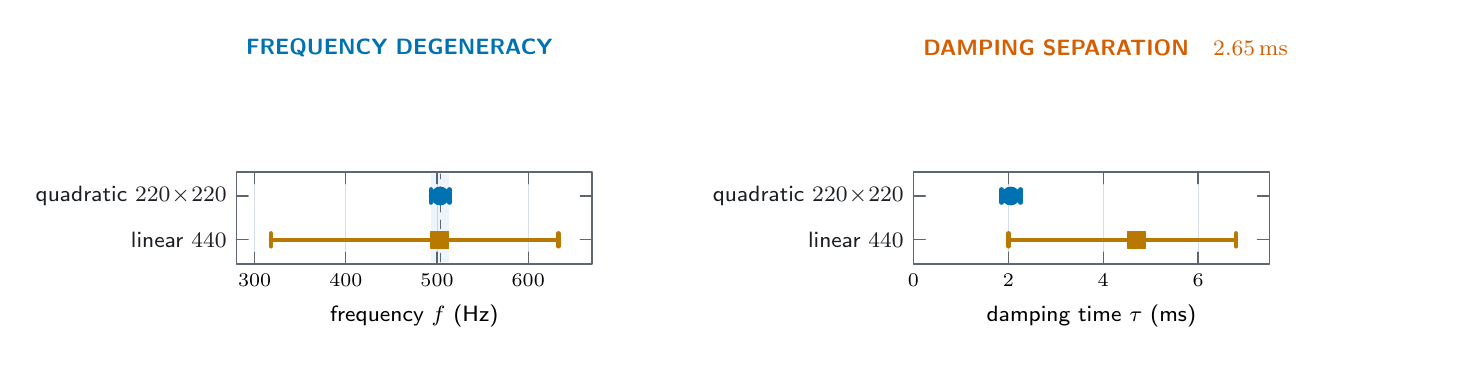
\begin{tikzpicture}[x=1cm,y=1cm,line cap=round,line join=round]
  \useasboundingbox (0,0) rectangle (17.80,4.15);
  \node[font=\sffamily\bfseries\footnotesize,text=qblue,anchor=west] at (2.65,3.89)
    {FREQUENCY DEGENERACY};
  \node[font=\sffamily\bfseries\footnotesize,text=qverm,anchor=west] at (11.25,3.89)
    {DAMPING SEPARATION\quad\normalfont $2.65\,\mathrm{ms}$};

  \begin{axis}[
    at={(2.65cm,1.15cm)},anchor=south west,
    width=6.10cm,height=2.75cm,
    xmin=280,xmax=670,ymin=-.55,ymax=1.55,
    xlabel={frequency $f$ (Hz)},
    label style={font=\sffamily\footnotesize},
    tick label style={font=\sffamily\scriptsize},
    xtick={300,400,500,600},ytick={0,1},
    yticklabels={linear $440$,quadratic $220\!\times\!220$},
    y tick label style={font=\sffamily\footnotesize,text=qink},
    xmajorgrids=true,major grid style={qgrid,line width=.35pt},
    axis line style={qmuted,line width=.45pt},tick style={qmuted,line width=.45pt},
    clip=false,
  ]
    \path[fill=qblue,opacity=.07]
      (axis cs:493.4,-.5) rectangle (axis cs:513.6,1.5);
    \draw[qmuted,dashed,line width=.45pt] (axis cs:503.4,-.5)--(axis cs:503.4,1.5);
    \draw[qgold,line width=1.55pt] (axis cs:318,0)--(axis cs:633,0);
    \draw[qgold,line width=1.55pt] (axis cs:318,-.15)--(axis cs:318,.15);
    \draw[qgold,line width=1.55pt] (axis cs:633,-.15)--(axis cs:633,.15);
    \addplot[only marks,mark=square*,mark size=3.15pt,qgold] coordinates {(503,0)};
    \draw[qblue,line width=1.65pt] (axis cs:493.4,1)--(axis cs:513.6,1);
    \draw[qblue,line width=1.65pt] (axis cs:493.4,.85)--(axis cs:493.4,1.15);
    \draw[qblue,line width=1.65pt] (axis cs:513.6,.85)--(axis cs:513.6,1.15);
    \addplot[only marks,mark=*,mark size=3.2pt,qblue] coordinates {(503.4,1)};
  \end{axis}

  \begin{axis}[
    at={(11.25cm,1.15cm)},anchor=south west,
    width=6.10cm,height=2.75cm,
    xmin=0,xmax=7.5,ymin=-.55,ymax=1.55,
    xlabel={damping time $\tau$ (ms)},
    label style={font=\sffamily\footnotesize},
    tick label style={font=\sffamily\scriptsize},
    xtick={0,2,4,6},ytick={0,1},
    yticklabels={linear $440$,quadratic $220\!\times\!220$},
    y tick label style={font=\sffamily\footnotesize,text=qink},
    xmajorgrids=true,major grid style={qgrid,line width=.35pt},
    axis line style={qmuted,line width=.45pt},tick style={qmuted,line width=.45pt},
    clip=false,
  ]
    \draw[qgold,line width=1.55pt] (axis cs:2.0,0)--(axis cs:6.8,0);
    \draw[qgold,line width=1.55pt] (axis cs:2.0,-.15)--(axis cs:2.0,.15);
    \draw[qgold,line width=1.55pt] (axis cs:6.8,-.15)--(axis cs:6.8,.15);
    \addplot[only marks,mark=square*,mark size=3.15pt,qgold] coordinates {(4.7,0)};
    \draw[qblue,line width=1.65pt] (axis cs:1.86,1)--(axis cs:2.26,1);
    \draw[qblue,line width=1.65pt] (axis cs:1.86,.85)--(axis cs:1.86,1.15);
    \draw[qblue,line width=1.65pt] (axis cs:2.26,.85)--(axis cs:2.26,1.15);
    \addplot[only marks,mark=*,mark size=3.2pt,qblue] coordinates {(2.05,1)};
  \end{axis}
\end{tikzpicture}
\end{document}
